% a simple template with cesbio color code

\documentclass[xcolor=table, t, aspectratio=169]{beamer} 
\graphicspath{{../FIGURES/}}
\usepackage[utf8]{inputenc}
\usepackage{booktabs, comment} 
\usepackage[absolute, overlay]{textpos} 
\usepackage{pgfpages}
\usepackage{caption}
\usepackage[font=footnotesize]{caption}
\usepackage{multirow}
\usepackage{hyperref}
\usepackage{blindtext}
\usepackage{amsmath}
\usepackage[makeroom]{cancel}
\usepackage{textpos}
\usepackage{tikz}
\usepackage{csquotes}
\usepackage{graphicx}


% CESBIO ADAPTED COLOURS 
\definecolor{colorLAERO}{RGB}{67, 141, 204}
\definecolor{forestgreen}{rgb}{0.13, 0.55, 0.13}
\definecolor{greenyellow}{rgb}{0.68, 1.0, 0.18}
\definecolor{inchworm}{rgb}{0.7, 0.93, 0.36}

% OPTIONAL COLOURS
% you can add the ones you need : lot of proposition on http://latexcolor.com/
\definecolor{ballblue}{rgb}{0.13, 0.67, 0.8}
\definecolor{bluegreen}{rgb}{0.0, 0.87, 0.87}
\definecolor{chromeyellow}{rgb}{1.0, 0.65, 0.0}
\definecolor{darkcyan}{rgb}{0.0, 0.55, 0.55}
\definecolor{darkpastelred}{rgb}{0.76, 0.23, 0.13}
\definecolor{electricgreen}{rgb}{0.0, 1.0, 0.0}
\definecolor{electriclime}{rgb}{0.8, 1.0, 0.0}
\definecolor{deepcarrotorange}{rgb}{0.91, 0.41, 0.17}
\definecolor{ganttblue}   {HTML}{2B6CB0}
\definecolor{ganttcyan}   {HTML}{2C7A7B}
\definecolor{ganttgreen}  {HTML}{276749}
\definecolor{ganttorange} {HTML}{C05621}
\definecolor{ganttgray}   {HTML}{4A5568}
\definecolor{ganttbg}     {HTML}{EBF4FF}
\definecolor{ganttbar}    {HTML}{BEE3F8}
\definecolor{milestonecol}{HTML}{E53E3E}


% CESBIO ADAPTED BEAMER OPTIONS
\setbeamercolor{title in head/foot}{bg=inchworm, fg=forestgreen}
\setbeamercolor{author in head/foot}{bg=colorLAERO}
\setbeamertemplate{page number in head/foot}{}

\useoutertheme{infolines}
\usetheme{Warsaw}
\usecolortheme[named=colorLAERO]{structure}


% SPECIFIC COMMANDS
% if you nee to set command for youe presentation, you can put them here
\newcommand{\defnotation}[1]{\bf{\textsl{#1}}}

\usepackage[
citestyle=abbrv, 
bibstyle=abbrv,
style=authoryear, %-comp,
backend=biber
%maxbibnames=99, % Make sure we are printing all authors in the appendix
]{biblatex}

\usepackage{pgfgantt}
\usepackage{helvet}
% PRESENTATION INFORMATIONS
% to fill in

% \title[]{}
% \subtitle{Subtitle}

\usetikzlibrary{positioning, calc}
\usetikzlibrary{calc}

% ── Colours (adapt to your theme) ─────────────────────────────────────────────
\definecolor{titleblue}  {HTML}{1A365D}
\definecolor{accentblue} {HTML}{2B6CB0}
\definecolor{lightgray}  {HTML}{EDF2F7}
\definecolor{medgray}    {HTML}{718096}

% ── Metadata ──────────────────────────────────────────────────────────────────
\author[J.~Hedman]{Johan Hedman}
\institute[LAERO]{Laboratoire d'Aérologie (LAERO) · Université de Toulouse}
\date{\today}

% ── Title frame ───────────────────────────────────────────────────────────────
% Use a fully custom frame instead of \titlepage for full layout control
\newcommand{\customtitleframe}{%
\begin{frame}[plain]
	\begin{tikzpicture}[remember picture, overlay]
		
		%% ── Background ─────────────────────────────────────────────────────────────
		\fill[titleblue]
		(current page.north west) rectangle
		($(current page.north east) + (0, -0.38\paperheight)$);
		
		\fill[accentblue]
		($(current page.north west) + (0, -0.38\paperheight)$) rectangle
		($(current page.north east) + (0, -0.405\paperheight)$);
		
		%% ── Title block ────────────────────────────────────────────────────────────
		\node[anchor=west, text=white, font=\large\bfseries, text width=0.95\paperwidth,] at 
		($(current page.north west) + (0.7cm, -0.13\paperheight)$)
		{Etude des rouleaux de couche limite sous les tempêtes};
		
		\node[anchor=west, text=white!70!titleblue, font=\small,text width=0.85\paperwidth,] at 
		($(current page.north west) + (0.7cm, -0.26\paperheight)$)
		{Johan Hedman \quad·\quad LAERO, Université de Toulouse \quad·\quad \insertdate};
		
		%% ── Supervisors ────────────────────────────────────────────────────────────
		\node[anchor=north west, font=\bfseries\small\color{accentblue}] at 
		($(current page.north west) + (0.7cm, -0.405\paperheight - 0.52cm)$)
		{Supervision};
		
		\node[anchor=north west, font=\footnotesize\color{titleblue}, align=left, text width=0.38\paperwidth]
		at ($(current page.north west) + (0.7cm, -0.405\paperheight - 1.0cm)$)
		{%
			\textbf{Prof. Jean-Pierre Chaboureau} \\
			\textcolor{medgray}{LAERO, Université de Toulouse} \\[5pt]
		};
		
		%% ── Divider ────────────────────────────────────────────────────────────────
		\draw[accentblue!30, line width=0.5pt]
		($(current page.north west) + (0.50\paperwidth, -0.405\paperheight - 0.50cm)$) --
		($(current page.south west) + (0.50\paperwidth, 0.45cm)$);
		
		%% ── Jury ───────────────────────────────────────────────────────────────────
		\node[anchor=north west, font=\bfseries\small\color{accentblue}]at ($(current page.north west) + (0.53\paperwidth, -0.405\paperheight - 0.52cm)$)
		{Membre du CSI};
		
		\node[anchor=north west, font=\footnotesize\color{titleblue}, align=left, text width=0.42\paperwidth]
		at ($(current page.north west) + (0.53\paperwidth, -0.405\paperheight - 1.0cm)$)
		{%
			\textbf{Prof } \textcolor{medgray}{\textit{}} \\
			\textbf{Prof.~Firstname Lastname} \textcolor{medgray}{\textit{}} \\
		};
		
		%% ── Logo strip ─────────────────────────────────────────────────────────────
		\fill[white]
		($(current page.south west) + (0, 0.10\paperheight)$)
		rectangle (current page.south east);
		
		\draw[accentblue!25, line width=0.4pt]
		($(current page.south west) + (0, 0.10\paperheight)$) --
		($(current page.south east) + (0, 0.10\paperheight)$);
		
		\node[anchor=south west, xshift=0.5cm, yshift=0.20cm] at (current page.south west)		{
\includegraphics[height=1.5cm]{LOGO/LAERO-logo.jpg}};
		
		\node[anchor=south, yshift=0.25cm] at (current page.south)
			{
\includegraphics[height=1.0cm]{LOGO/UNIV-logo.png}\hspace{1cm}%
			
\includegraphics[height=1.20cm]{LOGO/CNRS-logo.jpeg}};
		
		\node[anchor=south east, xshift=-0.5cm, yshift=0.20cm] at (current page.south east)
		{
\includegraphics[height=1.2cm]{LOGO/logo-IRD.png}};
		
	\end{tikzpicture}
\end{frame}
}





% cesbio adapted frame structure
\addtobeamertemplate{navigation symbols}{}{%
    \usebeamerfont{footline}%
    \usebeamercolor[fg]{footline}%
    \hspace{1em}%
    \insertframenumber/\inserttotalframenumber
}

\usepackage{soul}
\makeatletter
\let\HL\hl
\renewcommand\hl{%
  \let\set@color\beamerorig@set@color
  \let\reset@color\beamerorig@reset@color
  \HL}
\makeatother

\addbibresource{../../groupeThese.bib}
\graphicspath{{FIGURES/}}

%Title Page
\title{Réunion Mardi 27/01/2026}
\author{}

\usepackage[caption = false]{subfig}
\begin{document}
\begin{frame}
\maketitle
\end{frame}

\subsection{Dernière discussion}
\begin{frame}{Dernière discussion}
Ce qu'on avait dit
  \begin{itemize}
    \item \textbf{Intérêt d'introduire un forçage de grande échelle} : On veut un champ de large échelle qui comprend pas la petite échelle ! Forcer seulement le CCB et pas la couche limite ? (pas fait)
    \item rappel surement trop fort, $\tau$ à augmenter (pas fait)
    \item spectre ok on a pic pour rouleaux mais se déplace pou dx dim; pas de grde longueur d'onde
    \begin{figure}
    	   \centering
    	\begin{minipage}{.5\textwidth}
    		\centering
		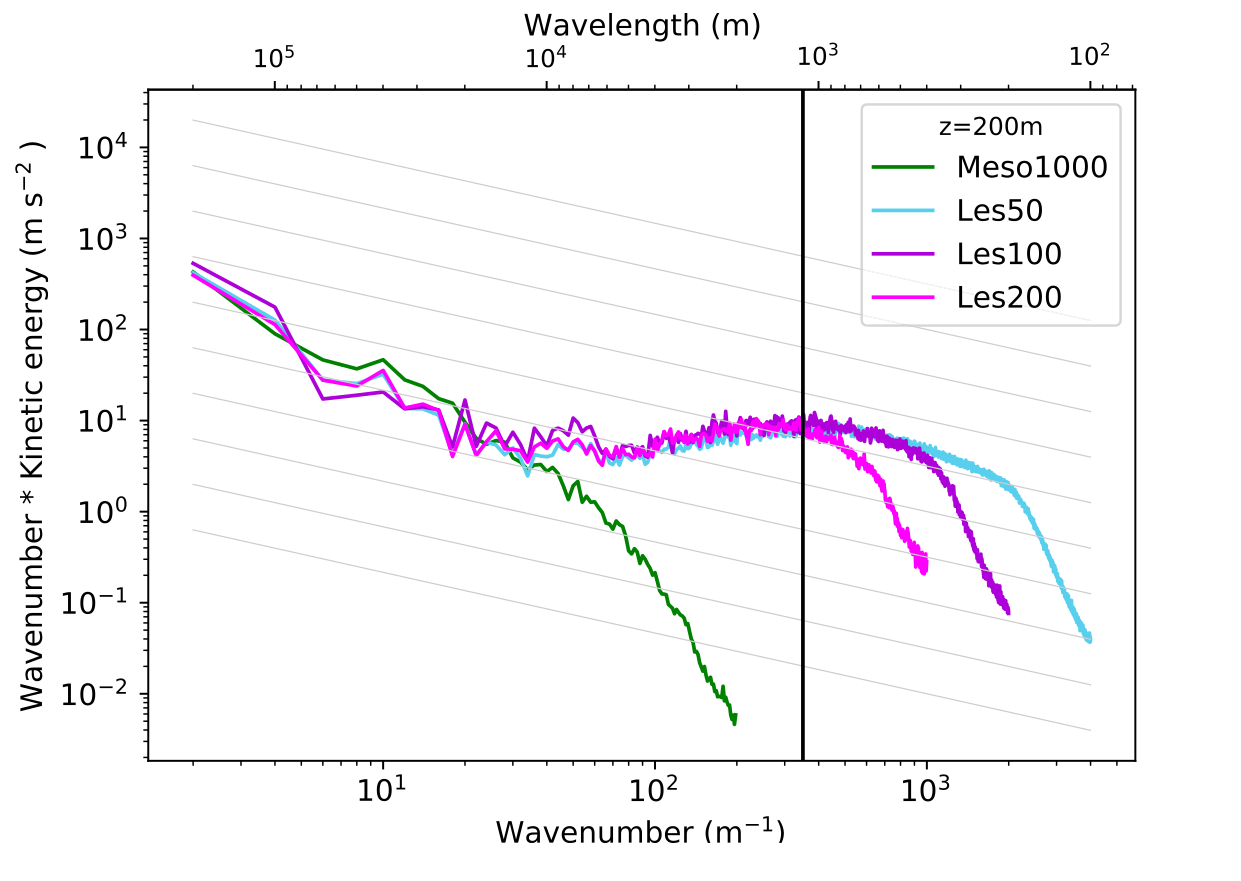
\includegraphics[width=0.9\textwidth]{spectre_LFAHR.png}
    	\end{minipage}%
    	\begin{minipage}{0.5\textwidth}
    		\centering
		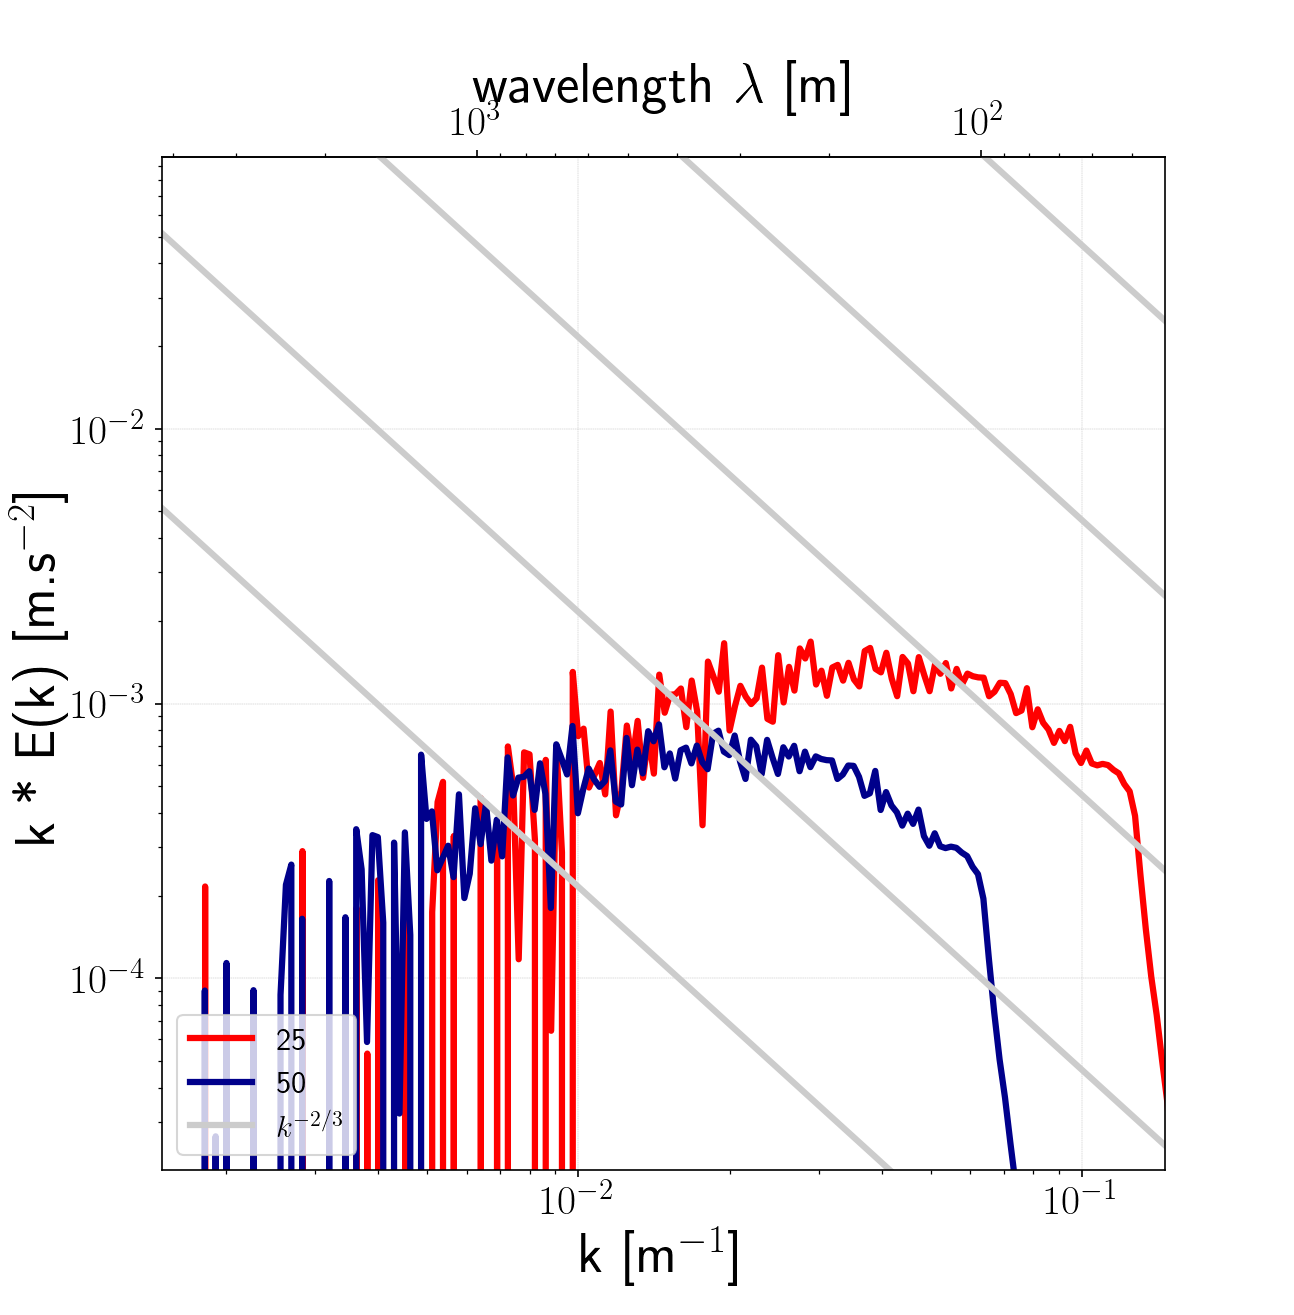
\includegraphics[width=0.6\textwidth]{spectre_MOI.png}
    	\end{minipage}

	\end{figure}
    
 \end{itemize}
\end{frame}

\begin{frame}{Retour réu MesoNH}
	\begin{itemize}
		\item Pk sur mer ?
    \item Influence de l'humidité
    \item $dz$ 

	\end{itemize}
\end{frame}

\subsection{Rapport simulation}
\begin{frame}{Travail sur simulation}
	\begin{itemize}
		\item Ajout de la vapeur d'eau, 1 g/kg (mais profil de Adrian?) \\
		+ schéma de micro physique : REVE
		\item Agrandissement taille de domaine : 10km x 10km x 1km ($\Delta z$ A AUGMENTER)
		\item Simualtion dvp couche limite en  LES en CAO \cite{chlondThreedimensionalSimulationCloud1992} : vents de 25m/s, grille cyclique 6 x 6 x 1.6 km, prise en compte condensation, rayonnement IR, subsidence de grande échelle, humidité de grande échelle, chauffage du sol(t)  
	\end{itemize}
\end{frame}


\begin{frame}{betterDOMAIN\_3D}
Pas de rouleaux	
\begin{figure}[h!]
	\centering
	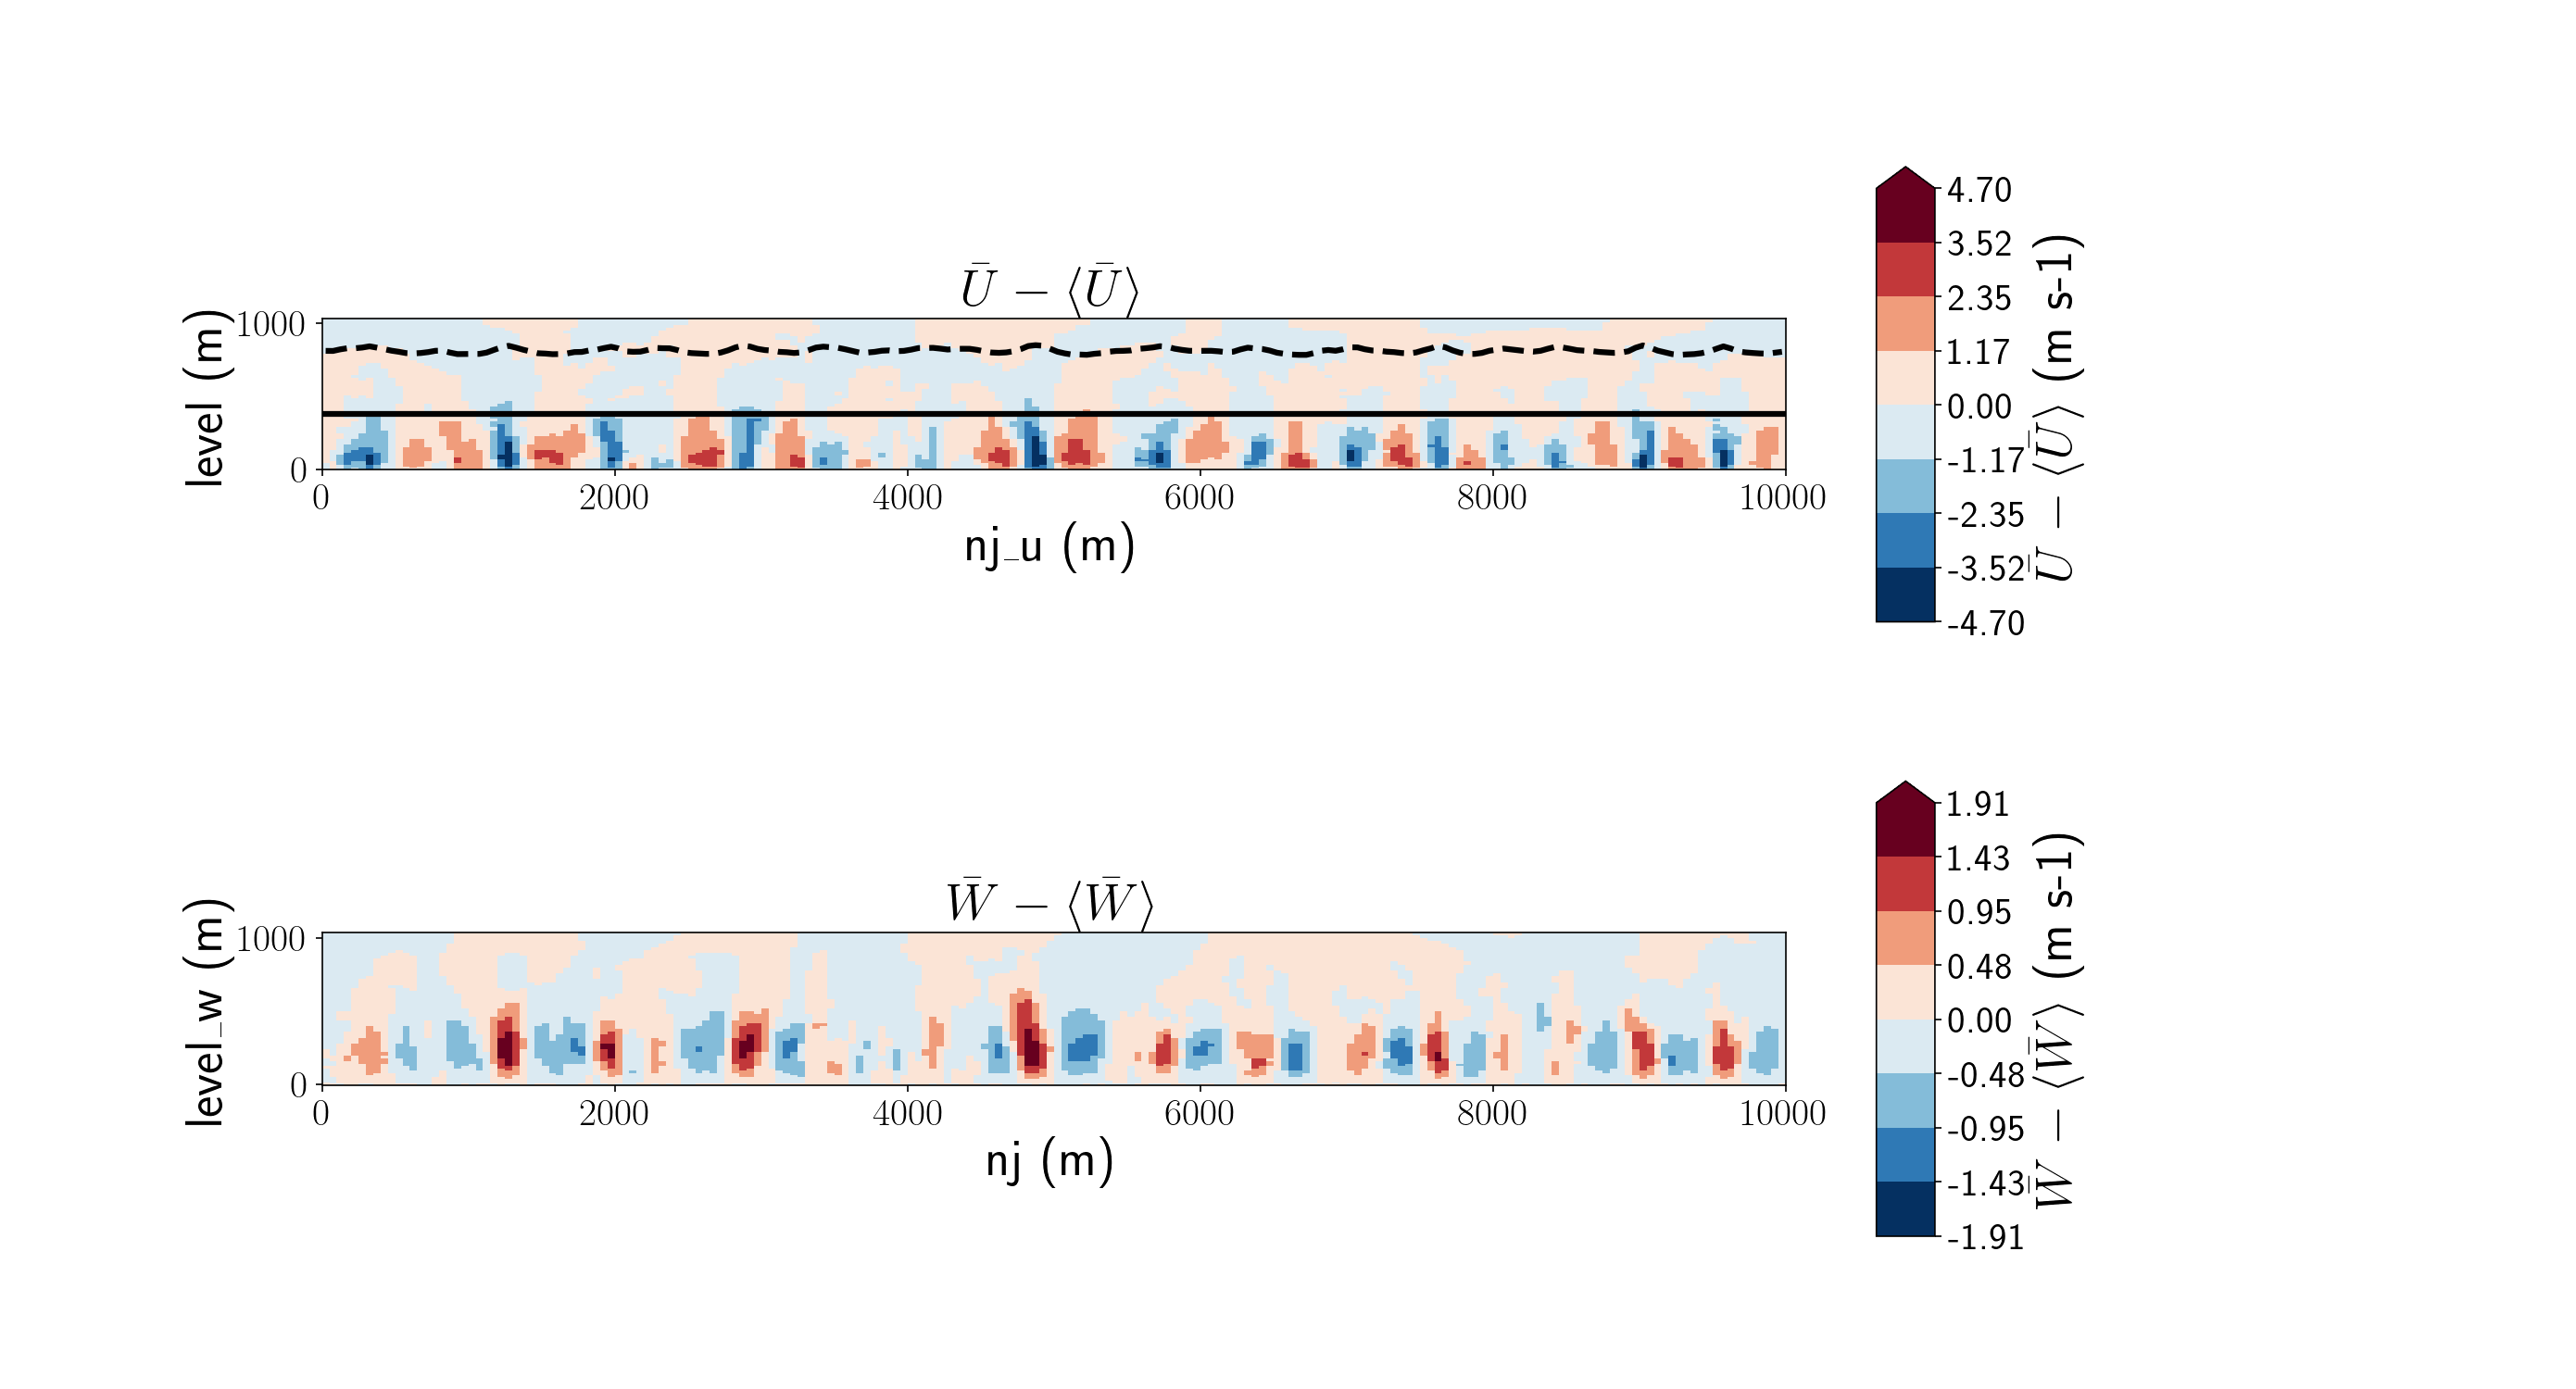
\includegraphics[width=0.7\textwidth]{rolls_ni_10_tmin20_tmax32.png}
	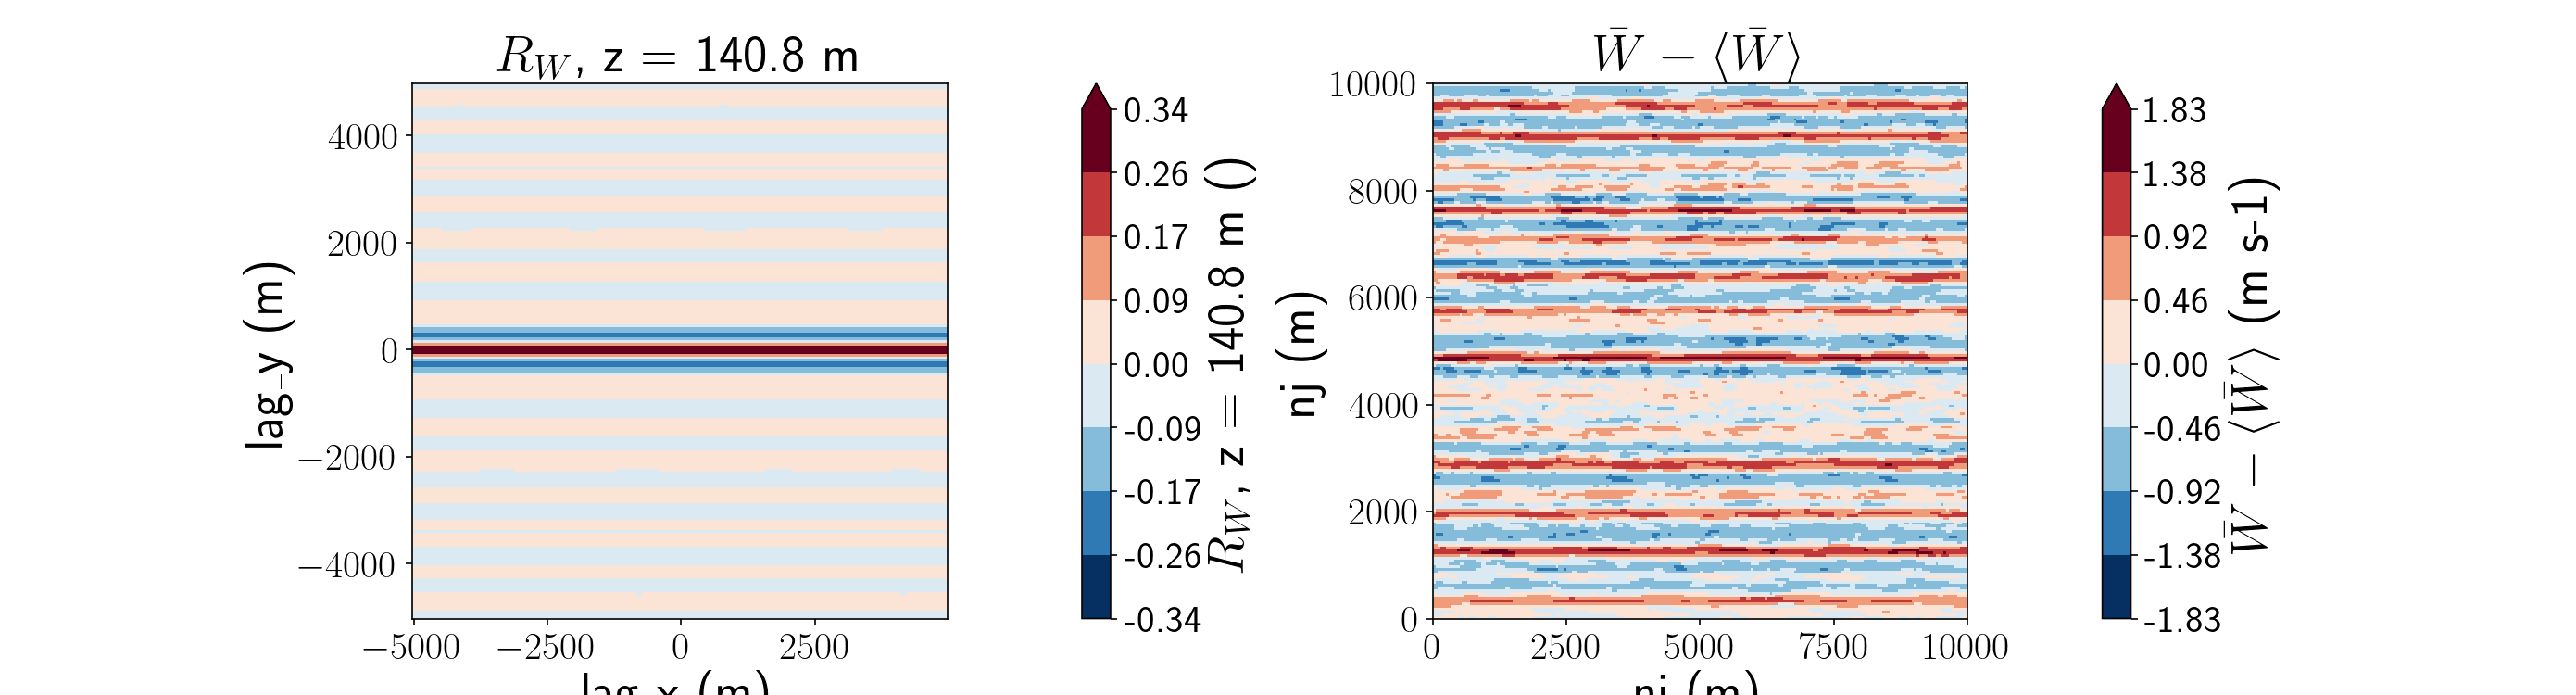
\includegraphics[width=0.8\textwidth]{R_autocorr_tmin20_tmax32.png}
\end{figure}
\end{frame}

\subsection{Suite}
\begin{frame}{Piste 1: Automatisation test}
	\begin{figure}[h!]
    	\centering
		
\includegraphics[width=0.7\textwidth]{projet.png}
	\end{figure}
\end{frame}

\begin{frame}{Piste 2: Cas idélaisé de Adrian suite}
\begin{itemize}
\item Quelle perturbation ? Influence de ce choix ? (dans \cite{chlondThreedimensionalSimulationCloud1992} perturbation temp au dernier niveau) 
\item Continuer de travailler sur ce cas mais il faut des profils. Possibilité sur l’Italie. \cite{giovanniniMultimodelConvectionresolvingSimulations2021}
\item Output de la simulation de Wahbiba ? 
\end{itemize}
\end{frame}
\end{document}   
